
Host-initiated memory ordering routines operate at single-thread granularity.

Ordering and completion in the presence of GPU-attached memory are defined with
respect to the two \emph{memory domains} exposed by each \ac{PE}---the default
(host) memory domain and the \ac{GPU} (device) memory domain
(\cref{subsec:memory_domains})---as shown in \cref{fig:mem-domains}.
\FUNC{shmem\_fence} orders the
delivery of operations to a given \ac{PE} within a single memory domain, whereas
\FUNC{shmem\_quiet} completes operations and makes them visible across both
memory domains at all \acp{PE}. \Cref{fig:fence-quiet} contrasts the two
routines.

\begin{figure}[!ht]
\centering
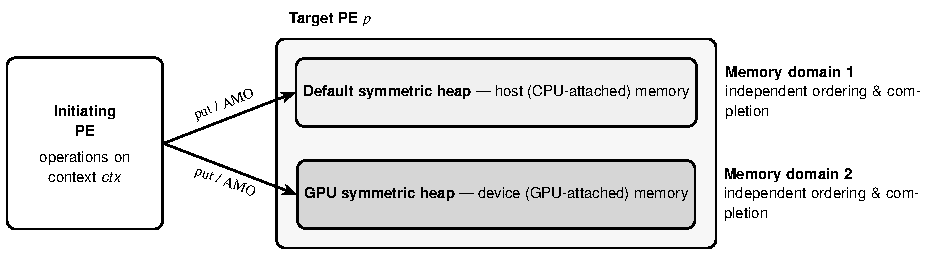
\includegraphics{figures/fig-mem-domains.pdf}
\caption{Each PE exposes two independent \emph{memory domains}: the default
symmetric heap in host (CPU-attached) memory and the GPU symmetric heap in device
(GPU-attached) memory. When GPU-aware communication is enabled, ordering and
completion are defined per memory domain: \FUNC{shmem\_fence} orders delivery
within one domain at a given PE, while \FUNC{shmem\_quiet} completes operations
and makes them visible across both domains at all PEs.}
\label{fig:mem-domains}
\end{figure}

\subsubsection{SHMEM\_FENCE}\label{subsec:ga_shmem_fence}

Ensures ordering of delivery of put, nonblocking get, \ac{AMO}, memory store, and put-with-signal
operations on symmetric data objects in the same memory domain when GPU-aware communication is enabled.

\begin{apidefinition}
\begin{Csynopsis}
void shmem_fence(void);
void shmem_ctx_fence(shmem_ctx_t ctx);
\end{Csynopsis}

\begin{apiarguments}
\apiargument{IN}{ctx}{A context handle specifying the context on which to perform
the operation. When this argument is not provided, the operation is performed on
the default context.}
\end{apiarguments}

\apidescription{
The \FUNC{shmem\_fence} routine ensures ordering of delivery of put, \ac{AMO},
memory store, and put-with-signal operations on symmetric data objects. All such
operations on symmetric data objects issued to a memory domain on a particular \ac{PE} on the given
context prior to the call to \FUNC{shmem\_fence} are guaranteed to be delivered
before any subsequent such operations to the same domain on the same \ac{PE} on the same context.
\FUNC{shmem\_fence} guarantees order of delivery, not completion. It does not
guarantee order of delivery of nonblocking get or values fetched by nonblocking
\ac{AMO} routines.

Memory store operations include direct stores to symmetric data objects performed
through local pointers returned by \FUNC{shmem\_ptr} or
\FUNC{shmem\_team\_ptr}. When the target symmetric data object resides in the
\ac{GPU} symmetric heap, a direct store through such a pointer constitutes a
memory store to the \ac{GPU} symmetric heap.

When GPU-aware communication is enabled, \FUNC{shmem\_fence} retains the
per-target-PE ordering semantics defined in \openshmem 1.6. However, when two
operations issued by the same \ac{PE} target different memory domains on the same
target \ac{PE}, \FUNC{shmem\_fence} does not provide cross-domain visibility
guarantees.

If \VAR{ctx} has the value \CONST{SHMEM\_CTX\_INVALID}, no operation is
performed.
}

\apireturnvalues{
None.
}

\apinotes{
\FUNC{shmem\_fence} only provides per-PE ordering guarantees and does not
guarantee completion of delivery. When GPU-aware communication is in use,
\FUNC{shmem\_fence} is sufficient to order operations that target the same memory
domain on the same \ac{PE}. It is not sufficient to guarantee visibility when two
operations target different memory domains on the same \ac{PE}.

The \FUNC{shmem\_quiet} routine should be called if completion of put, \ac{AMO},
memory store, or put-with-signal operations on symmetric data objects is desired
when operations target different memory domains or when multiple target \acp{PE}
are involved.
}
\end{apidefinition}

\subsubsection{SHMEM\_QUIET}\label{subsec:ga_shmem_quiet}

Waits for completion of all outstanding put, \ac{AMO}, memory store, and
put-with-signal operations on symmetric data objects issued by a \ac{PE} when
GPU-aware communication is enabled.

\begin{apidefinition}
\begin{Csynopsis}
void shmem_quiet(void);
void shmem_ctx_quiet(shmem_ctx_t ctx);
\end{Csynopsis}

\begin{apiarguments}
\apiargument{IN}{ctx}{A context handle specifying the context on which to perform
the operation. When this argument is not provided, the operation is performed on
the default context.}
\end{apiarguments}

\apidescription{
The \FUNC{shmem\_quiet} routine ensures completion of all outstanding put,
\ac{AMO}, memory store, and put-with-signal operations on symmetric data objects
issued by the calling \ac{PE} on the given context. All such operations are
guaranteed to be complete and visible to all \acp{PE} when \FUNC{shmem\_quiet}
returns.

When GPU-aware communication is enabled, \FUNC{shmem\_quiet} ensures completion
and visibility of all prior operations to both the default symmetric heap and the
\ac{GPU} symmetric heap at their respective targets. The receiving \ac{PE} shall
perform appropriate host-device synchronization after observing data that
indicates completion before accessing data from a prior operation that resides in
GPU-attached memory.

If \VAR{ctx} has the value \CONST{SHMEM\_CTX\_INVALID}, no operation is
performed.
}

\apireturnvalues{
None.
}

\apinotes{
There is a subtle difference between \FUNC{shmem\_fence} and
\FUNC{shmem\_quiet}, in that \FUNC{shmem\_quiet} guarantees completion of all
operations on symmetric data objects, making the updates visible to all other
\acp{PE} across all memory domains, including the \ac{GPU} symmetric heap and the
default symmetric heap. \FUNC{shmem\_fence} provides only per-PE ordering within
a single memory domain and does not guarantee cross-domain visibility.
}
\end{apidefinition}

\begin{figure}[!ht]
\centering
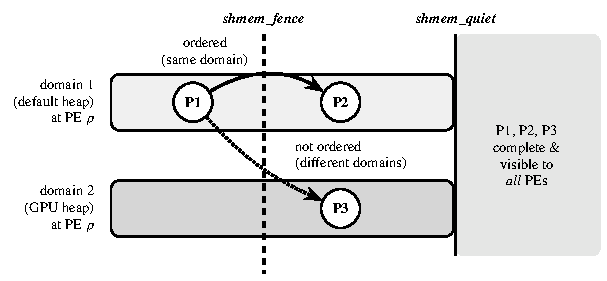
\includegraphics{figures/fig-fence-quiet.pdf}
\caption{Memory-domain-based ordering and completion. \FUNC{shmem\_fence}
guarantees that operations issued before it are delivered before operations
issued after it \emph{when they target the same memory domain at the same PE}
(P1 before P2). It provides no ordering between operations that target different
memory domains at the same PE (P1 and P3), and none across different PEs.
\FUNC{shmem\_quiet} completes all prior operations and makes them visible to all
PEs across both memory domains.}
\label{fig:fence-quiet}
\end{figure}

\subsubsection{SHMEM\_PUT\_SIGNAL}\label{subsec:ga_put_signal_ordering}

Copies data from a contiguous local data object to a data object on a specified
\ac{PE} and subsequently updates a remote flag to signal completion. The
put-with-signal routines guarantee ordering between the data delivery and the
signal update within a single operation, including when the data and the signal
target different memory domains.

\begin{apidefinition}
\begin{Csynopsis}
void shmem_put_signal(TYPE *dest, const TYPE *source, size_t nelems,
    uint64_t *sig_addr, uint64_t signal, int sig_op, int pe);
void shmem_ctx_put_signal(shmem_ctx_t ctx, TYPE *dest, const TYPE *source,
    size_t nelems, uint64_t *sig_addr, uint64_t signal, int sig_op, int pe);
\end{Csynopsis}

\begin{apiarguments}
\apiargument{IN}{ctx}{A context handle specifying the context on which to perform
the operation.}
\apiargument{OUT}{dest}{Symmetric address of the data object to be updated on the
remote PE.}
\apiargument{IN}{source}{Local address of the data object containing the data to
be copied.}
\apiargument{IN}{nelems}{Number of elements in the \VAR{dest} and \VAR{source}
arrays.}
\apiargument{OUT}{sig\_addr}{Symmetric address of the signal data object to be
updated on the remote PE as a signal.}
\apiargument{IN}{signal}{Unsigned 64-bit value used for updating the remote
\VAR{sig\_addr}.}
\apiargument{IN}{sig\_op}{Signal operator for the update on \VAR{sig\_addr}.}
\apiargument{IN}{pe}{PE number of the remote PE.}
\end{apiarguments}

\apidescription{
When GPU-aware communication is enabled, the \VAR{dest} data object and the
\VAR{sig\_addr} signal data object may reside in different memory domains on the
same target \ac{PE}. The \VAR{dest} data object may reside in the \ac{GPU}
symmetric heap and the \VAR{sig\_addr} signal data object may reside in the
default symmetric heap, or the reverse. The put-with-signal routine guarantees
that the data is delivered to the \VAR{dest} data object before the signal update
is visible at the \VAR{sig\_addr} signal data object, regardless of whether the
two objects reside in the same or different memory domains.

This cross-domain ordering guarantee is specific to the put-with-signal routine.
It does not extend to ordering between a put-with-signal routine and other
independent operations.
}

\apireturnvalues{
None.
}

\apinotes{
Unlike the case where two independent operations target different memory domains,
the put-with-signal routine provides cross-domain ordering between its data
delivery and signal update as a single atomic-like operation.
\FUNC{shmem\_fence} does not provide equivalent cross-domain ordering for two
independent operations.
}
\end{apidefinition}

\begin{figure}[!ht]
\centering
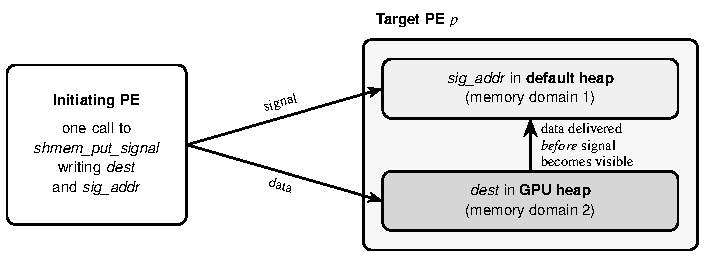
\includegraphics{figures/fig-put-signal-xdomain.pdf}
\caption{Cross-domain ordering of \FUNC{shmem\_put\_signal}. A single
put-with-signal operation guarantees that the data written to \textit{dest} is
delivered before the signal update at \textit{sig\_addr} becomes visible, even
when \textit{dest} and \textit{sig\_addr} reside in different memory domains at
the target PE. Two independent operations ordered with \FUNC{shmem\_fence} do
not provide this cross-domain guarantee.}
\label{fig:put-signal-xdomain}
\end{figure}

\subsubsection{Global Synchronization}\label{subsec:ga_barrier}

\begin{apidefinition}
\begin{Csynopsis}
void shmem_barrier_all(void);
void shmem_barrier(int PE_start, int logPE_stride, int PE_size, long *pSync);
\end{Csynopsis}

\begin{apiarguments}
\apiargument{IN}{PE\_start}{The lowest PE number of the active set of PEs.}
\apiargument{IN}{logPE\_stride}{The log (base 2) of the stride between
consecutive PE numbers in the active set.}
\apiargument{IN}{PE\_size}{The number of PEs in the active set.}
\apiargument{IN}{pSync}{Symmetric address of a work array of size at least
\CONST{SHMEM\_BARRIER\_SYNC\_SIZE}.}
\end{apiarguments}

\apidescription{
When GPU-aware communication is enabled, the implicit completion semantics of
\FUNC{shmem\_barrier\_all} and \FUNC{shmem\_barrier} are equivalent to calling
\FUNC{shmem\_quiet} on the default context prior to synchronization. All prior
operations to both the default symmetric heap and the \ac{GPU} symmetric heap are
guaranteed to be complete and visible to all \acp{PE} when the barrier returns,
regardless of whether the operations target different memory domains or different
\acp{PE}.
}

\apireturnvalues{
None.
}

\apinotes{
The \FUNC{shmem\_barrier\_all} routine is equivalent to calling
\FUNC{shmem\_ctx\_quiet} on the default context followed by calling
\FUNC{shmem\_team\_sync} on the world team.

The \FUNC{shmem\_team\_sync} routine, in contrast with the barrier routines, only
ensures completion and visibility of previously issued memory stores and does not
ensure completion of remote memory updates issued through \openshmem routines.
}
\end{apidefinition}

